\documentclass[9pt,twocolumn,twoside]{pnas-new}
% Use the lineno option to display guide line numbers if required.
% Note that the use of elements such as single-column equations
% may affect the guide line number alignment. 

\templatetype{pnasresearcharticle} % Choose template 
% {pnasresearcharticle} = Template for a two-column research article
% {pnasmathematics} = Template for a one-column mathematics article
% {pnasinvited} = Template for a PNAS invited submission
\usepackage{siunitx}


\setboolean{displaywatermark}{false} % Set to false to remove the watermark

\title{Bestimmung der Spurabstände von optischen Datenträger}

% Use letters for affiliations, numbers to show equal authorship (if applicable) and to indicate the corresponding author
\author[a]{Armin Beck}
\author[a]{André Berberich} 
\author[a]{Fabian Konrad}

\affil[a]{Student der DHBW Mosbach}


% Keywords are not mandatory, but authors are strongly encouraged to provide them. If provided, please include two to five keywords, separated by the pipe symbol, e.g:
\keywords{Laser $|$ CD $|$ DVD $|$ Storage} 

\begin{abstract}
This paper presents a revolutionary and repeatable method to prove the track pitch of an optical, laser based, data medium.
Using a hand held light emitting pistol, the track pitch of an standard medium was measured to be between 0,73 \si{\micro\metre} and 1,6 \si{\micro\metre}.
Results show outstanding agreement with the provided, theoretical values of the manufacturers.
The method presented has significant implications for future storage of big data in the cloud 
and may one day will be the contributing factor for the digitization of the industry.
\end{abstract}

\dates{This manuscript was compiled on \today}

\begin{document}

% Optional adjustment to line up main text (after abstract) of first page with line numbers, when using both lineno and twocolumn options.
% You should only change this length when you've finalised the article contents.
\verticaladjustment{-2pt}

\maketitle
\thispagestyle{firststyle}
\ifthenelse{\boolean{shortarticle}}{\ifthenelse{\boolean{singlecolumn}}{\abscontentformatted}{\abscontent}}{}
.
\dropcap{D}ie Forschung ist sich einig, dass es wichtig ist, bestehende Technologien zu reflektieren und daraus entsprechende Schlüsse für die Zukunft zu ziehen. Weiterentwicklungen im Speicherbereich dienen als Grundlage für den Weg der Digitalisierung, und der globalen Vernetzung. 
Die Anforderungen an Speicher, der jederzeit erreichbar, redundant ausgelegt und hochperformant sein muss, steigt mit jedem Tag.
Auch Privatanwender sind von diesem \glqq recht abrupte[n] Paradigmenwechsel\grqq \space betroffen \cite[Heft 10/2012 S.102]{CT1990}.
Die in diesem Artikel vorgestellte Methode ermöglicht es Spurabstände auf optischen Datenträgern mit einfachsten Mitteln zu bestimmen und zu validieren ohne hierbei einen Computer oder ein Laufwerk zu verwenden. Dadurch wird man in die Lage versetzt, die siginfikanten Unterschiede diverser optischer Medien im Bezug auf die Datenkapazität, zu erklären.
Die mit dieser Vorgehensweise ermittelten Werte für handelsübliche CDs und DVDs, sollen als Referenz und Denkanstoß für die Entwicklung von innovativen Speicherlösungen von morgen dienen.

\section*{Technische Grundlagen für den Versuch}
Bei diesem Versuch nimmt man sich die bei einem von elektromagnetischen Wellen bestrahlten Doppelspalt auftretetenden Effekte zur Hilfe. Wird eine Lochplatte beziehungsweise eine Spaltplatte von einem Laserstrahl getroffen, so verteilt sich das Licht nahezu gleichmäßig hinter der Spaltplatte. Hält man eine Mattscheibe hinter den Doppelspalt, erscheinen mehrere von der Mitte aus in zunehmendem Abstand symmetrisch angeordnete Punkte. Dies würde eigentlich einer gleichmäßigen Verteilung widersprechen. Die Besonderheit ist jedoch, dass zwei Spalten verwendet werden und daher der Lichtstrahl an Beiden gestreut wird. Betrachtet man nun einen Punkt in einem Abstand von beiden Löchern, der sich um jeweils %n\times\varlambda
unterscheidet, ist an diesem die Bestrahlungsstärke höher, da die aus beiden Spalten austretenden Wellen an dieser Stelle nicht zueinander phasenverschoben sind. ein sogenanntes Interferenzmaximum entsteht aus der Addition der Amplituden beider austretender Wellen. An anderen Stellen tritt eine Phasenverschiebung auf, da die Lichtstrahle an unterschiedlichen Punkten der Periode zusammentreffen. Somit entsteht eine von der Position abhängige stehende Welle, die durch die Mattscheibe visualisiert wird.

\subsection*{Aufbau und Leseverfahren einer CD und einer DVD}
CDs und DVDs bestehen grundsätzlich aus drei Schichten. Die Unterste Schicht ist eine Kunststoffscheibe, auf der die binären Daten in Form vom Löchern im Mikrometerabstand eingeprägt, mit einem starken Laser eingebrannt oder eingeäzt wurden. Ein Loch steht für das Signal 1 und eben kein Loch stellt die 0 dar. Die zweite Schicht ist eine Aluminium- oder Goldfolie, die der Unterseite ihre typische Färbung verleiht. Als dritte Schicht wir eine bedruckte Schutzfolie oben aufgeklebt.Beim Lesen der CD, genauso wie  beim Lesen einer DVD tritt keine Interferenz auf, da das Lasersignal so stark gebündelt is, dass es nur ein einziges Loch auf einmal trifft. Bei diesen Disks wird das auftreffende Licht mit Hilfe der darüber liegenden Folie gespiegelt. An der Stelle, auf die das Licht zurückgestrahlt werden würde, wenn der aktuell bestrahlte Abschnitt der Disk nicht eingeprägt wäre, befindet sich ein Sensor, der seine Bestrahlungsstärke misst. Jedes mal, wenn der Laserstrahl auf ein Loch in der sich drehenden Disk trifft, wird dieses an eine andere als die ursprüngliche Stelle hin gespiegelt und es kommt kein Signal am Empfänger an. Dieser erzeugt somit eine 1 als Ausgangssignal. Anderenfalls erzeugt er eine 0.

\section*{Versuchsaufbau}

\begin{figure}[!htbp]
\centering
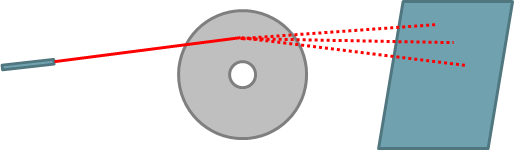
\includegraphics[width=0.3\textwidth,keepaspectratio]
{Pictures/Versuchsaufbau.png}
\parbox{0.9\textwidth}

{\caption{\label{fig:Versuchsaufbau}
Schematischer Aufbau}
\sffamily \small{Versuchsaufbau}
}
\end{figure}
\subsection*{Interferenz / Versuchsergebnisse}

 Da der Lochabstand von CD und DVD extrem gering ist, kann man diese mit einem handelsüblichen Laserpointer durchleuchten und hierbei die Löcher als Doppelspalt verwenden. Es treten die oben genannten Effekte auf, anhand deren man das Verhältnis aus Wellenlänge und Lochabstand berechnen kann.


\section*{Interpretation der ermittelten Werte}
Durch die gewonnen Messergebnisse aus [... Referenz zu Messergebnisse] konnten die Hersteller Angaben von 0,73 \si{\micro\metre} (DVD) \cite{ECMA1300} und  1,6 \si{\micro\metre} (CD) \cite{ECMA359} bestätigt werden.
\begin{equation} \label{eq:cdspur} S_{\mbox{cd}} =  1,62\mbox{ \textmu m}  \end{equation}
\begin{equation} \label{eq:dvdspur} S_{\mbox{dvd}} =  0,73\mbox{ \textmu m}  \end{equation} 
\subsection{Vergleich Datenkapazität CD und DVD}
Der geringere Spurabstand der DVD ist einer der Gründe, warum diese eine höhere Datenkapazität als CD hat, obwohl beide die gleiche Bauform haben.

\begin{figure}[!htbp]
\centering
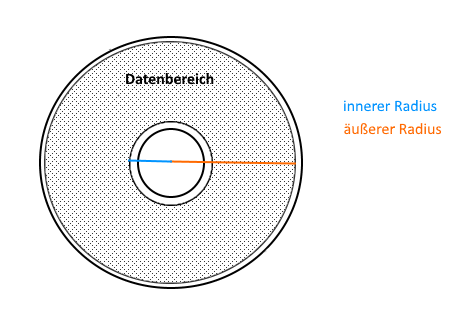
\includegraphics[width=0.5\textwidth,keepaspectratio]
{Pictures/Rohling.png}
\parbox{0.9\textwidth}

{\caption{\label{fig:Rohling}
Schematische Darstellung einer CD/DVD}

\sffamily \small{Ein typischer Rohling mit gekennzeichnetem Datenbereich und Radien}
}
\end{figure}

Aus \ref{fig:Rohling}, das den schematischen Aufbau einer CD oder DVD zeigt, können zwei Radien entnommen werden, über die die Fläche des Datenbereichs berechnet werden kann.
Für die folgenden Berechnungen gilt:  \begin{math} r_{\mbox{i}}  = \mbox{innerer Radius und } r_{\mbox{a}} = \mbox{äußerer Radius} \end{math} \\
Von einer CD konnten die folgenden Werte abgelesen werden: \begin{math} r_{\mbox{inner}_{\mbox{cd}}} = 2,3 \mbox{ cm und } r_{\mbox{outer}_{\mbox{cd}}} = 5,8 \mbox{ cm} \end{math} \\

Mit der Formel für die Fläche eines Kreisringes \cite[Seite 147]{Bartsch2014} kann die Fläche für Daten berrechnet werden: \begin{equation} \label{eq:kreisring} A = \pi((r_a)^2-(r_i)^2)  \end{equation} 

Die Gesamtlänge einer Spur kann folgendermaßen berechnet werden \begin{equation} \label{eq:gesamtlänge} L = \frac{\mbox{Fläche für Daten}}{\mbox{Spurbreite}} \end{equation}
Die Anzahl der Bits im Datenbereich kann dann anschließend ebenfalls berechnet werden \begin{equation} \label{eq:bitanzahl} N_{bits} = \frac{L}{0,5*\mbox{Spurbreite}} \end{equation}

\subsection{Berechnung CD}
Für eine CD ergibt sich folgende Berechnung: \\ \\
Für die genutzte Datenfläche aus \eqref{eq:kreisring}
\begin{align*}
 A_{cd} &= \pi\cdot((r_{\mbox{outer}_{\mbox{cd}}})^2-(r_{\mbox{inner}_{\mbox{cd}}})^2)  \ref{eq:kreisring}\\	
&= \pi\cdot((5,8\mbox{cm})^2-(2,3\mbox{ cm})^2) \\
 &=  \pi\cdot((0,0058\mbox{ m})^2-(0,0023\mbox{ m})^2) \approx  8,91\cdot10^{-3}\mbox{ m}^2.
\end{align*}

Für die Gesamtlänge der Spur aus \ref{eq:kreisring} ergibt sich mit \eqref{eq:cdspur}
\begin{align*}
 L_{cd} &= \frac{\mbox{Fläche für Daten}}{\mbox{Spurbreite}}\\
 &= \frac{A_{\mbox{cd}}}{S_{\mbox{cd}}}\\
 &= \frac{8,91\cdot10^{-3}\mbox{ m}^2}{1,62\cdot10^{-6}\mbox{ m} }\\
 &= 5500\mbox{ m}
\end{align*}

Die Anzahl der Bits beträgt dann über \eqref{eq:bitanzahl}
\begin{align*}
N_{\mbox{cd-bits}} &=  \frac{L_{\mbox{cd}}}{0,5\cdot s_{\mbox{cd}}}\\
&= \frac{5500\mbox{ m}}{0,5 \cdot 1,62 \cdot 10^{-6}\mbox{ m}}\\
&= 6790123457 \\
&\approx 6,79 \cdot 10^9
\end{align*}

Umgerechnet in MByte
\begin{align*}
C_{\mbox{cd}} &= \frac{N_{\mbox{cd-bits}}}{8\cdot1024\cdot1024}\\
&= \frac{ 6,79\cdot10^9}{8\cdot1024\cdot1024}\\
&\approx 809\mbox{ MB}
\end{align*}

Die Größenordnung entspricht der einer handelsüblichen CD.

\subsection{Berechnung DVD}
Für eine DVD ergibt sich analog dazu die folgende Berechnung: \\ \\
Von einer DVD konnten die folgenden Werte abgelesen werden: \begin{math} r_{\mbox{inner}_{\mbox{dvd}}} = 2,3 \mbox{ cm und } r_{\mbox{outer}_{\mbox{dvd}}} = 5,9 \mbox{ cm} \end{math} \\

Für die genutzte Datenfläche aus \eqref{eq:kreisring}
\begin{align*}
 A_{\mbox{dvd}} &= \pi\cdot((r_{\mbox{outer}_{\mbox{dvd}}})^2-(r_{\mbox{inner}_{\mbox{dvd}}})^2)  \ref{eq:kreisring}\\	
&= \pi\cdot((5,9\mbox{cm})^2-(2,3\mbox{ cm})^2) \\
 &=  \pi\cdot((0,0059\mbox{ m})^2-(0,0023\mbox{ m})^2) \approx 9,27\cdot10^{-3}\mbox{ m}^2.
\end{align*}

Für die Gesamtlänge der Spur aus \ref{eq:kreisring} ergibt sich mit \eqref{eq:cdspur}
\begin{align*}
 L_{\mbox{dvd}} &= \frac{\mbox{Fläche für Daten}}{\mbox{Spurbreite}}\\
 &= \frac{A_{\mbox{dvd}}}{S_{\mbox{dvd}}}\\
 &= \frac{9,27\cdot10^{-3}\mbox{ m}^2}{0,73\cdot10^{-6}\mbox{ m} }\\
 &\approx 12700\mbox{ m}
\end{align*}

Die Anzahl der Bits beträgt dann über \eqref{eq:bitanzahl}
\begin{align*}
N_{\mbox{dvd-bits}} &=  \frac{L_{\mbox{dvd}}}{0,5\cdot S_{\mbox{dvd}}}\\
&= \frac{12700\mbox{ m}}{0,5\cdot 0,73\cdot10^{-6}\mbox{ m}}\\
&\approx 3,48\cdot 10^{10}
\end{align*}

Umgerechnet in GByte
\begin{align*}
C_{\mbox{dvd}} &= \frac{N_{\mbox{dvd-bits}}}{8\cdot1024\cdot1024}\\
&= \frac{3,48\cdot10^{10}}{8\cdot1024\cdot1024\cdot1024}\\
&\approx 4,05\mbox{ GB}
\end{align*}

Auch diese Größenangabe entspricht der einer handelsübliche DVD.


Mit dieser Methode ist es nun auch möglich, weitere optische Datenträger zu überprüfen.
Aufgrund der erhebbaren Daten sind Neuerungen in der Speichertechnik von optische Medien denkbar, die in der Zukunft eine zentrale Rolle für Speicherlösungen spielen können.
Denkbar sind extrem kleine Spurabstände oder Medien, die sehr viele verschiedene Datenspuren enthalten.


% \pnasbreak splits and balances the columns before the references.
% Uncomment \pnasbreak to view the references in the PNAS-style
% If you see unexpected formatting errors, try commenting out \pnasbreak
% as it can run into problems with floats and footnotes on the final page.
%\pnasbreak

% Bibliography
\bibliography{ReferenceDatabase}


\end{document}